%\documentclass[12pt, a4paper, oneside, titlepage, final]{book}
\documentclass[12pt, a4paper, twoside, titlepage, final]{book}
\renewcommand{\familydefault}{\sfdefault}
%\documentclass[12pt,a4paper,onecolumn,oneside,11pt,wide,floatssmall]{book}

\usepackage{polski}
\usepackage[utf8]{inputenc}
\usepackage[OT4]{fontenc}


\linespread{1.3}								% 1.3 do interlinii 1.5


% w�asne pakiety

%===============================================================================
% Ustawienia dokumentu

\frenchspacing

% ustawienia wymiar�w


\oddsidemargin 20mm							% margines nieparzystych stron
\evensidemargin 20mm							% margines parzystych stron
%\headheight 15pt								% wysoko�� paginy g�rnej
%\topmargin 20mm									% margines g�rny

% styl paginacji
\pagestyle{fancy}
%\renewcommand{\chaptermark}[1]{\markboth{#1}{}}
%\renewcommand{\sectionmark}[1]{\markright{\thesection\ #1}{}}

% nag��wek 
\fancyhf{}
\fancyfoot[LE,RO]{\thepage}
\fancyhead[C]{\small\nouppercase{\rightmark}}

%\fancyhead[R]{\small\nouppercase{\leftmark}}
\renewcommand{\headrulewidth}{0.1pt}
\renewcommand{\footrulewidth}{0pt}

% nag��wek w stylu plain 
\fancypagestyle{plain}
{
\fancyhf{}
\renewcommand{\headrulewidth}{0pt}
\renewcommand{\footrulewidth}{0pt}
}

% ta sekwencja tworzy czyste kartki na stronach po \cleardoublepage
\makeatletter
\def\cleardoublepage{\clearpage\if@twoside \ifodd\c@page\else
	\hbox{}
	\vspace*{\fill}
	\thispagestyle{empty}
	\newpage
	\if@twocolumn\hbox{}\newpage\fi\fi\fi}
\makeatother

%===============================================================================
% Zmienne �rodowiskowe i polecenia

% definicja
\newtheorem{definition}{Definicja}[chapter]

% twierdzenie
\newtheorem{theorem}{Twierdzenie}[chapter]

% obcoj�zyczne nazwy
\newcommand{\foreign}[1]{\emph{#1}}

% pozioma linia
\newcommand{\horline}{\noindent\rule{\textwidth}{0.4mm}}

% wstawianie obrazk�w {plik}{caption}{opis}


%===============================================================================
% ustawienia pakietu hyperref

\hypersetup{
    colorlinks,
    citecolor=black,
    filecolor=black,
    linkcolor=black,
    urlcolor=blue
}
\hypersetup
{
%colorlinks=true,			% false: boxed links; true: colored links
%linkcolor=black,			% color of internal links
%citecolor=black,			% color of links to bibliography
%filecolor=black,			% color of file links
%urlcolor=black			% color of external links
}
			% do³¹czanie plików stylu
\usepackage{pwtitle}
\usepackage{multirow}
\usepackage{tocloft}
\usepackage{chngcntr}
\usepackage{varwidth}
\usepackage{indentfirst}
\usepackage{polski}
\usepackage{float}
\usepackage[utf8]{inputenc}
\usepackage{listings}
%\usepackage{slashbox}
%\usepackage[table]{xcolor}
\usepackage{graphicx,pdflscape}
\usepackage{placeins}
\usepackage[final]{pdfpages}
\usepackage{longtable}

%\input{listing.tex}
\counterwithout{figure}{chapter}
\counterwithout{equation}{chapter}
\lstset{
  numberbychapter=false,
	extendedchars=true
}
%\counterwithout{lstlisting}{chapter}

\usepackage{titlesec}

\titleformat{\chapter}{\sffamily\huge\bf}{\thechapter.}{20pt}{\huge\bf}
%\usepackage{geometry}
\begin{document}
\hyphenation{Par-tial-ac-ti-vi-ty}
\hyphenation{zwra-ca}
\hyphenation{get-Ho-ri-zon-tal-View-Angle}

%===============================================================================
% Front

\frontmatter

%\frontmatter

%\frontmatter

%\frontmatter

%\input{front.tex}
\input{front//biography.tex}
\input{front//mark.tex}
\input{front//summary.tex}
\input{front//statement.tex}
\input{front//dedication.tex}
{\tableofcontents}

	\newpage
	\thispagestyle{empty}

\begin{flushright}

  \begin{varwidth}[t]{\textwidth}
	Kierunek studiów: Telekomunikacja\\
	Specjalność: Telekomunikacja \\
	Numer albumu: 236501\\
	Data urodzenia: 04.02.1991 \\
	Data rozpoczęcia studiów: 01.10.2014 \\
  \end{varwidth}

\end{flushright}
	\vspace*{\stretch{1}}

\begin{center}
    \textbf{\textbf{Życiorys}}
\end{center}

	\vspace{0.5cm}

Urodziłem się 4 lutego 1991 roku w Olsztynie.
W roku 2010 uzyskałem tytuł finalisty LXI Olimpiady Matematycznej oraz
ukończyłem II Liceum Ogólnokształcące im. Konstantego Ildefonsa Gałczyńskiego w Olsztynie.
W tym samym roku rozpocząłem studia na Politechnice Warszawskiej na kierunku Elektronika, Informatyka i Telekomunikacja.
Od 2011 roku współpracowałem z prof. T. Łubą oraz dr inż. G. Borowikiem w ramach koła Eksploracji Danych.
W czasie studiów dwukrotnie zdobyłem stypendium rektora za wyniki w nauce.
Przez rok na przełomie 2013 i 2014 roku pracowałem jako Java Developer w firmie IMPAQ.
Po ukończeniu stódiów inżynierskich w październiku 2014 rozpocząłem studia drugiego stopnia.
Od marca 2015 łączyłem studia z pracą na stanowisku Android Developer w firmie El Passion.

	\vspace{1cm}

\begin{flushright}
	\begin{minipage}{5cm}
		\dotfill \\[-0.7cm]
		\begin{center}
		\small Podpis
		\end{center}
	\end{minipage}
\end{flushright}

	\vspace{2cm}

\newpage
	\thispagestyle{empty}
\begin{flushleft}
    	\begin{minipage}{11cm}
		Egzamin dyplomowy: \\
		Złożył egzamin dyplomowy w dniu: \dotfill \\
		z wynikiem: \dotfill \\
		Ogólny wynik studiów: \dotfill \\
		Dodatkowe uwagi i wnioski Komisji: \dotfill \\
		\dotfill
	\end{minipage}
\end{flushleft}
\newpage
\vspace{10cm}

\newpage
\begin{center}
	\textbf{Synteza funkcji generowania indeksów metodą redukcji i kompresji argumentów}
\end{center}
\noindent{\textbf{Streszczenie}}

Funkcje boolowskie można realizować w~ukłądach programowalnych przy użyciu pamięci adresowanych.
Problemem, który się pojawia, jest rozmiar tych pamięci.
Zaprezentowany w~niniejszej pracy algorytm generowania funkcji indeksów skutecznie ogranicza ten problem.
Korzysta on z faktu,
że wiele funkcji boolowskich o~$n$ argumentach i $k$ wierszach może być reprezentowana przy pomocy mniejszej liczby argumentów,
jeżeli $k<<2^n$.
Proponowane rozwiązanie,
korzystające z istniejących algorytmów syntezy logicznej,
zmniejsza liczbę argumentów wymaganych do reprezentacji funkcji.

\textit{\textbf{Słowa kluczowe:}} funkcja generowania indeksów; dekompozycja liniowa; redukcja atrybutów; eksploracja danych; minimalne pokrycie kolumnowe.

	\vspace{1cm}

\begin{center}
    \textbf{Index generation function based on argument reduction and linear function decomposition}
\end{center}
\noindent{\textbf{Summary}}

Boolean functions can be realised in field-programmable utilising address memory.
However for large functions memory size can be insufficient.
The thesis provides an index generation function algorithm to address this issue.
Many boolean functions with $n$ arguments and a~weight of $k$ can be represented using fewer than $n$ arguments if only $k<<2^n$ condition occurs.
Suggested solution uses existing logic synthesis algorithms to reduce set of attributes required in function realisation.

\textit{\textbf{Keywords:}} index generation function; linear decomposition; argument reduction; data exploration; unate covering.

	\vspace*{\stretch{1}}

\newpage
\thispagestyle{empty}

\vspace*{\stretch{1}}

\begin{center}
\LARGE\textsc{Oświadczenie}
\end{center}

\vspace{1cm}

Oświadczam, że Pracę Dyplomową pod tytułem \emph{,,Synteza funkcji generowania indeksów metodą redukcji i~kompresji argumentów''}, którą kierował prof. dr hab. inż. Tadeusz Łuba, wykonałem samodzielnie, co poświadczam własnoręcznym podpisem.

\vspace{2cm}

\begin{flushright}
\begin{minipage}{5cm}
	\dotfill \\[-0.7cm]
	\begin{center}
	\small{Karol Kowalski}
	\end{center}
\end{minipage}
\end{flushright}

\vspace*{\stretch{1}}

\newpage
\thispagestyle{empty}
\vspace*{\stretch{1}}
\begin{flushright}
\textit{Składam serdeczne podziękowania
panu prof. dr hab. inż. Tadeuszowi Łubie
za pomoc w trakcie przygotowywania pracy.}
\end{flushright}
{\tableofcontents}

	\newpage
	\thispagestyle{empty}

\begin{flushright}

  \begin{varwidth}[t]{\textwidth}
	Kierunek studiów: Telekomunikacja\\
	Specjalność: Telekomunikacja \\
	Numer albumu: 236501\\
	Data urodzenia: 04.02.1991 \\
	Data rozpoczęcia studiów: 01.10.2014 \\
  \end{varwidth}

\end{flushright}
	\vspace*{\stretch{1}}

\begin{center}
    \textbf{\textbf{Życiorys}}
\end{center}

	\vspace{0.5cm}

Urodziłem się 4 lutego 1991 roku w Olsztynie.
W roku 2010 uzyskałem tytuł finalisty LXI Olimpiady Matematycznej oraz
ukończyłem II Liceum Ogólnokształcące im. Konstantego Ildefonsa Gałczyńskiego w Olsztynie.
W tym samym roku rozpocząłem studia na Politechnice Warszawskiej na kierunku Elektronika, Informatyka i Telekomunikacja.
Od 2011 roku współpracowałem z prof. T. Łubą oraz dr inż. G. Borowikiem w ramach koła Eksploracji Danych.
W czasie studiów dwukrotnie zdobyłem stypendium rektora za wyniki w nauce.
Przez rok na przełomie 2013 i 2014 roku pracowałem jako Java Developer w firmie IMPAQ.
Po ukończeniu stódiów inżynierskich w październiku 2014 rozpocząłem studia drugiego stopnia.
Od marca 2015 łączyłem studia z pracą na stanowisku Android Developer w firmie El Passion.

	\vspace{1cm}

\begin{flushright}
	\begin{minipage}{5cm}
		\dotfill \\[-0.7cm]
		\begin{center}
		\small Podpis
		\end{center}
	\end{minipage}
\end{flushright}

	\vspace{2cm}

\newpage
	\thispagestyle{empty}
\begin{flushleft}
    	\begin{minipage}{11cm}
		Egzamin dyplomowy: \\
		Złożył egzamin dyplomowy w dniu: \dotfill \\
		z wynikiem: \dotfill \\
		Ogólny wynik studiów: \dotfill \\
		Dodatkowe uwagi i wnioski Komisji: \dotfill \\
		\dotfill
	\end{minipage}
\end{flushleft}
\newpage
\vspace{10cm}

\newpage
\begin{center}
	\textbf{Synteza funkcji generowania indeksów metodą redukcji i kompresji argumentów}
\end{center}
\noindent{\textbf{Streszczenie}}

Funkcje boolowskie można realizować w~ukłądach programowalnych przy użyciu pamięci adresowanych.
Problemem, który się pojawia, jest rozmiar tych pamięci.
Zaprezentowany w~niniejszej pracy algorytm generowania funkcji indeksów skutecznie ogranicza ten problem.
Korzysta on z faktu,
że wiele funkcji boolowskich o~$n$ argumentach i $k$ wierszach może być reprezentowana przy pomocy mniejszej liczby argumentów,
jeżeli $k<<2^n$.
Proponowane rozwiązanie,
korzystające z istniejących algorytmów syntezy logicznej,
zmniejsza liczbę argumentów wymaganych do reprezentacji funkcji.

\textit{\textbf{Słowa kluczowe:}} funkcja generowania indeksów; dekompozycja liniowa; redukcja atrybutów; eksploracja danych; minimalne pokrycie kolumnowe.

	\vspace{1cm}

\begin{center}
    \textbf{Index generation function based on argument reduction and linear function decomposition}
\end{center}
\noindent{\textbf{Summary}}

Boolean functions can be realised in field-programmable utilising address memory.
However for large functions memory size can be insufficient.
The thesis provides an index generation function algorithm to address this issue.
Many boolean functions with $n$ arguments and a~weight of $k$ can be represented using fewer than $n$ arguments if only $k<<2^n$ condition occurs.
Suggested solution uses existing logic synthesis algorithms to reduce set of attributes required in function realisation.

\textit{\textbf{Keywords:}} index generation function; linear decomposition; argument reduction; data exploration; unate covering.

	\vspace*{\stretch{1}}

\newpage
\thispagestyle{empty}

\vspace*{\stretch{1}}

\begin{center}
\LARGE\textsc{Oświadczenie}
\end{center}

\vspace{1cm}

Oświadczam, że Pracę Dyplomową pod tytułem \emph{,,Synteza funkcji generowania indeksów metodą redukcji i~kompresji argumentów''}, którą kierował prof. dr hab. inż. Tadeusz Łuba, wykonałem samodzielnie, co poświadczam własnoręcznym podpisem.

\vspace{2cm}

\begin{flushright}
\begin{minipage}{5cm}
	\dotfill \\[-0.7cm]
	\begin{center}
	\small{Karol Kowalski}
	\end{center}
\end{minipage}
\end{flushright}

\vspace*{\stretch{1}}

\newpage
\thispagestyle{empty}
\vspace*{\stretch{1}}
\begin{flushright}
\textit{Składam serdeczne podziękowania
panu prof. dr hab. inż. Tadeuszowi Łubie
za pomoc w trakcie przygotowywania pracy.}
\end{flushright}
{\tableofcontents}
			% definicja strony tytu³owej

%===============================================================================
% Rozdzia³y - dla porz¹dku pliki dla ka¿dego z rozdzia³ów znajduj± siê w oddzielnych katalogach
\mainmatter
\newgeometry{inner=40mm, outer=20mm}

\chapter{Wstęp}

W dzisiejszych czasach gromadzimy ogromne ilości danych.
W związku obserwujemy rozwój dziedziny eksploracji i~analizy danych
Pewna część tych problemów jest ściśle związana z~koniecznością precyzyjnego wyodrębniania właściwych danych z~ogromnej masy danych niepotrzebnych
Szczególnym przypadkiem analizy danych są dane binarne, reprezentowane wektorami binarnymi o~stosunkowo dużej liczbie bitów,
a małej liczbie danych które trzeba wyselekcjonować.
Jeżeli na dodatek zbiór danych selekcjonowanych podlega częstym zmianom,
to strukturę sprzętową takich układów trzeba często zmieniać.
W związku z~tym rozwiązaniem tego problemu są struktury FPGA z~wbudowanymi pamięciami ROM.
Ale kolejną barierą w~realizacji tych układów są ograniczenia w~nadmiernej pojemności pamięci ROM o~dużej liczbie wejść – np. 40,
co byłoby wymagane przy selekcji niewielkiej liczby wektorów (wzorców), np. 10.
Można jednak przypuszczać, że binarna tablica takich wektorów: 40 kolumn oznaczanych $x_1,…,x_{40}$ i~10 wierszy zawiera kolumny $x_i, x_j, ..., x_k$,
które ustawione obok siebie reprezentują różne liczby binarne \cite{sasao-workshop}.
Zwykle takich kolumn jest wyraźnie mniej od liczby zmiennych (bitów) wektorów selekcjonowanych.
Zatem jedną z~metod rozwiązania zadania selekcji jest redukcja argumentów,
a cały problem jest określany mianem syntezy funkcji generowania indeksów.

Zagadnienie redukcji argumentów jest tożsame z~problemem redukcji atrybutów.
W tym ujęciu zagadnienie to było badane bardzo intensywnie \cite{fast-algorithm, efektywna-procedura, new-reduction, steinbach-posthoff, skowron-rauszer, slezak, novel-method}.
Jednym z~najbardziej znanych algorytmów redukcji atrybutów jest algorytm zastosowany w~systemie RSES \cite{rses}.
Algorytm ten został skutecznie usprawniony w~pracy inżynierskiej \cite{efektywna-procedura},
natomiast w~ramach niniejszej pracy stworzono realizację obliczającą jedno rozwiązanie [rozdz. ??].
Analogiczne zadanie podjęto w~zespole prof. Sasao,
a w~referacie \cite{sasao-workshop} znaczenie redukcji zasygnalizowano informacją,
iż opracowanie algorytmu redukcji jest jednym z~najważniejszych zadań.

Drugim aktualnym zagadnieniem syntezy logicznej w~projektowaniu generatorów adresu jest dekompozycja liniowa.
Przez dekompozycję liniową rozumie się dekompozycję $F = H(G1, G2, ...,  X)$,
w której składowymi dekompozycji G są dwuargumentowe funkcje $EXOR$:
\begin{equation}
F = H (x_i \oplus x_j, x_k \oplus x_l, ..., X)
\end{equation}
Do najbardziej znanych algorytmów dekompozycji liniowej stosowanej w~generatorach adresów należy algorytm s-min \cite{sasao-recent, sasao-s-min}.
W artykule \cite{redukcja-kompresja} wykazano, że algorytm s-min jest mało skuteczny i~zaproponowano całkowicie inne ujęcie tego zagadnienia.
W niniejszej pracy metodykę tę przystosowano do heurystycznych obliczeń funkcji generowania indeksów.
Cechą charakterystyczną tej propozycji jest zastosowanie twierdzenia wiążącego dekompozycję liniową z~tzw. zbiorem rozróżnialności [rozdz. ??].
W rezultacie opracowano metodykę oraz algorytm (i jego implementację) do heurystycznych obliczeń praktycznych funkcji indeksowania [rozdz. …].
Przykłady takich dekompozycji podano w~rozdz. ??.

\section{Problem generowania indeksów w~technice cyfrowej}

Problem generowania indeksów (adresu) dotyczy szczególnie tej podgrupy problemów czasu rzeczywistego,
w których warunki podejmowania decyzji są zmienne w~czasie.
Sztandarowym zastosowaniem algorytmów generowania indeksów jest obsługa pakietów w~routerach IP.
Spotykamy się tam z~problemami filtrowania ruchu z~niepożądanych adresów (firewall) lub wybierania portów wyjściowych (routing).
W obu przypadkach znajdują zastosowanie struktury programowalne FPGA lub EEPROM
ze względu na połączenie szybkości działania porównywalnej z~rozwiązaniami ASIC oraz elastyczności jak w~przypadku rozwiązań programowych.
Wyzwania,
jakie są stawiane przed algorytmami generowania indeksów,
są związane częstymi zmianami danych.Indeksy często muszą być generowane w~czasie rzeczywistym wraz ze zmianami danych.
Ponadto ze względu na dużą liczbę argumentów,
które muszą być brane pod uwagę (32 bity - adresy IPv4, 48 bitów - adresy mac),
wymagane są optymalizacje pozwalające wykorzystywać pamięci dostępne w~strukturach programowalnych.
Przykładowo przy funkcji o~$n=6$ argumentach wszystkich wektorów binarnych jest 64 ($2^6$).
Jeżeli spośród wszystkich wektorów poszukiwanych jest $k=6$ konkretnych, wtedy dla każdego z~64 wektorów musielibyśmy przechować 3 bity ($\log_26$).
Dla takiego przykładu minimalna potrzebna pamięć to 192 bity.
Jednak dla mechanizmu znajdowania sygnatur wirusów składającego się z~$k=1\,300\,000$ poszukiwanych wektorów o~$n=40$ argumentach, taka pamięć miałaby rozmiar 21 terabitów.
\begin{multline} \\
2^n \cdot \log_2 k = \\
= 2^{40} \cdot \log_2 1\,300\,000 = \\
= 2^{10} \cdot 2^{10} \cdot 2^{10} \cdot 2^{10} \cdot 21 = \\
=21 \cdot 2^{10} \cdot 2^{10} \cdot 2^{10} k = \\
=21 \cdot 2^{10} \cdot 2^{10} M = \\
=21 \cdot 2^{10} G = \\
=21 [Tbit] \\
\end{multline}


\section{Zastosowania}
- Tablica trasowania
- Terminal access controller
- Memory patch circuit
- Skanowanie wirusów
- Dystrybucja adresów IP
- Skanowanie wirusów
- Wykrywanie niepożądanych danych
- Konwersja kodów

\subsection{Tablica trasowania}
W Internecie powszechne jest zagadnienie znajdowania ścieżek dla pakietów IP.
Każdy węzeł sieci przechowuje informacje dotyczące wyboru trasy dla przychodzących pakietów.
Dla każdego przechowywanego adresu IP w~tablicy adresów znajduje się indeks pamięci, w~którym przechowywane są wszystkie szczegóły.
Liczba adresów w~takiej pamięci wynosi nierzadko nawet 40 tysięcy.
Jako że adresy IP są reprezentowane przez 32 bity, tyle właśnie jest argumentów funkcji.
Dodatkowo w~wielu routerach mamy do czynienia z~dynamicznymi protokołami trasowania, które wymagają częstych zmian w~tablicy adresów.
Jest to w~związku z~tym bardzo dobry przykład zastosowania funkcji generowania indeksów.


\section{Algorytm Sasao}
Rozwiązanie problemu nadmiernej pojemności pamięci o~$n$ wejściach adresowych przy wykrywaniu $k$ wekrtorów indeksowanych ($k<<2^n$),
spośród $2^n$ możliwych wektorów wejściowych,
zaproponował Sasao \cite{sasao-workshop, sasao-recent, sasao-s-min, sasao-synthesis}.
Istotą tego rozwiązania jest
\begin{enumerate}[label=\alph*)]
\item Obliczanie minimalnej liczby argumentów potrzebnych do reprezentacji funkcji specyfikowanej $k$ wektorami $n$-bitowymi,
\item Dekompozycja liniowa funkcji obliczonej w~punkcie a)
\end{enumerate}

Dekompozycja liniowa polega na łączeniu argumentów w~grupy i~podawaniu ich na wejście dwu lub więcej argumentowych bramek XOR.
Algorytm s-Min, profesora Sasao, znajduje takie grupy.
Istnieją jednak przykłady,
dla których wskazanie żadnego takiego zbioru argumentów nie jest możliwe,
lub występuje ich mało w~stosunku do całkowitej liczby argumentów.
Z tego powodu częscią algorytmu Sasao są przekształcenia linowe,
mające na celu zwiększenie dostępnej liczby grup do dekompozycji bramkami XOR.
Dla funkcji ,,1 z~20'' (tabela numer \ref{fig:1of20}),
posiadającej $n=20$ argumentów oraz $k=20$ wierszy,
algorytm Sasao,
dla różnych wersji s-Min,
uzyskuje wynik kompresji argumentów od 14 do 8.

\begin{table}
\centering
\includegraphics[width = 13cm]{chapter01/1of20.png}
\caption{Przygład funkcji 1 z~20 (Źródło własne).}
\label{fig:1of20}
\end{table}

Z punktu widzenie syntezy funkcji generowania indeksów propozycja Sasao jest jak najbardziej prawidłowa.
Niestety zastosowany w~tej metodzie algorytm redukcji argumentów,
jak też prcedura obliczania dekompozycji liniowej nie są najskuteczniejsze.
Nowa metoda powstała na podstawie istniejących algorytmów z~dziedziny syntezy logicznej,
dla tego samego przykładu osiąga kompresję do 6 argumentów.
Tym samym pozwala wykorzysywać mniejsze i~tańsze urządzenie do rozwiązywania tych samych problemów,
albo na obsługę przoblemów, które wcześniej były zbyt zlożone,
za pomocą do tej pory używanego sprzętu komputerowego.

%Idea stojąca za takim rozwiązaniem bierze się stąd, że do rozróżnienia 1.3 miliona wektorów z~poprzedniego przykładu może wystarczyć jedynie 21 bitów.
%Gdyby udało się faktycznie zredukować liczbę wejść z~40 do 21 bitów, rozmiar pamięci zmniejszyłby się z~21 terabitów do 42 megabitów.
%\begin{multline} \\
%2^{21} \cdot \log_2 1300000 = \\
%= 2^{10} \cdot 2^{10} \cdot 2 \cdot 21 = 42 [Mbit] \\
%\end{multline}
%Zmniejszenie rozmiaru pamięci głównej nie pozwalałoby na jednoznaczne określenie czy dany wektor jest wektorem poszukiwanym.
%Wskazywałoby jedynie numer jedynego wiersza z~poszukiwanych, który ma szansę być identyczny z~wektorem sprawdzanym.
%Potrzebne jest zatem przechowanie wszystkich kompletnych wektorów poszukiwanych w~drugiej pamięci.
%W naszym przykładzie wektorów jest 1,3 miliona i~każdy ma 40 bitów.
%Rozmiar dodatkowej pamięci wyniósłby w~takim razie 50 megabitów.


%W zaproponowanym rozwiązaniu częścią, która ma największe znaczenie na rozmiar niezbędnej pamięci,
%jest wyznaczenie funkcji pozwalającej na jak największe zmniejszenie liczby wejść do głównej pamięci.
%\textbf{(Wymaga uzupełnienia z~artykułem)} W~pracy Profesora Sasao dla konkretnej funkcji ten wynik pozwala na ograniczenie wejść z~\textbf{N do X}.
%Sposobem zaproponowanym w~pracy uzyskujemy zmniejszenie z~\textbf{N do Y}.
%Warto zauważyć, że zmniejszenie o~jeden argument powoduje dwukrotne zmniejszenie wymaganej pamięci.



%\section{Cel pracy - do usunięcia}
%
%Celem pracy było opracowanie algorytmu generowania indeksów na podstawie istniejących algorytmów z~dziedziny syntezy logicznej
%oraz porównanie nowej metody z~wynikami aktualnych prac badawczych z~zakresu generowania indeksów.
%Wyniki obliczeń dla przykładu referencyjnego,
%przeprowadzone przed przystąpieniem do właściwych badań,
%potwierdziły konkurencyjność algorytmu opartego na połączeniu redukcji argumentów oraz dekompozycji liniowej.
%W porównaniu z~aktualnymi artykułami Profesora Sasao,
%nowa metoda pozwala na zmniejszenie zużycia zasobów potrzebnych do realizacji funkcji w~strukturach programowalnych.
%Tym samym pozwala wykorzysywać mniejsze i~tańsze urządzenie do rozwiązywania tych samych problemów,
%albo na obsługę przoblemów, które wcześniej były zbyt zlożone,
%za pomocą do tej pory używanego sprzętu komputerowego.

\chapter{Redukcja argumentów}

Algorytm generowania indeksów zaproponowany przez profesora Sasao,
pozwala na zastosowanie pamięci o mniejszym rozmiarze niż wskazywałaby na to liczba argumentów.
Nie jest to oczywiście jedyna metoda pozwalająca na  uzyskanie takiego efektu.
W tej pracy przedstawione zostało podejście wykorzystujące jednocześnie redukcję i kompresję argumentów.

Redukcja argumentów jest to proces pozwalający na zmniejszenie liczby parametrów wejściowych funkcji,
poprzez odrzucenie argumentów zawierających wyłącznie redundantne dane.
Po wykonaniu takiego procesu,
usunięcie dowolnego argumentu z funkcji powoduje kolizję wierszy o różnych wartościach i tym samym utratę informacji.
Zbiór argumentów powstały w wyniku redukcji nazywamy reduktem.
Istnieje wiele sposobów redukcji argumentów,
zarówno systematycznych,
pozwalających na znalezienie wszystkich minimalnych rozwiązań,
jak i heurystycznych,
charakteryzujących się szybszym działaniem.
Sama redukcja nie zawsze przynosi spektakularne rezultaty.
W skrajnych przypadkach funkcji,
w których każdy argument dostarcza niewielkiej,
ale niezbędnej porcji informacji,
redukcja może nie przynieść żadnego efektu.
W takich przypadkach niezbędna jest,
opisana w dalszej części pracy,
kompresja argumentów,
świetnie sprawdzająca się właśnie w takich przypadkach.

\section{Problem złożoności}

Do problemu redukcji argumentów można podejść w sposób intuicyjny.
Można próbować po kolei usuwać argumenty i weryfikować spójność danych.
W przypadku utraty spójności taki argument musiałby się znaleźć w końcowym rozwiązaniu.
W przeciwnym przypadku należałoby go usunąć i kolejne weryfikacje przeprowadzać z jego wyłączeniem.
Pojedyncza weryfikacja wymaga porównania,
każdych dwóch wierszy o różnej wartości funkcji.
Jeżeli funkcja ma $n$ argumentów oraz $m$ wierszy wtedy porównanie dwóch dowolnych wierszy odbywa się ze złożonością liniową $n$.
Par wierszy do porównania jest w zależności od rozkładu wartości funkcji od $m$ do $m^2$.
Zatem złożoność obliczeniowa pojedynczej weryfikacji to $n \cdot m^2$.
Taką weryfikację trzeba przeprowadzić dla każdego z $n$ argumentów co daje końcową złożoność $n^2 \cdot m^2$.

Problem takiego podejścia,
poza złożonością,
leży dodatkowo w jakości uzyskiwanego rozwiązania.
W procesie redukcji argumentów część z nich może być ważniejsza
i tym samym pozostawienie takiego argumentu może pozwolić na usunięcie dwóch (lub nawet więcej) innych.
Innymi słowami wynik takiej redukcji,
mimo że jest prawidłowy,
często jest nieoptymalny.

\section{Minimalne pokrycie kolumnowe}

Innym sposobem wyboru argumentów w czasie redukcji jest dobieranie argumentów,
aż do zapewnienia pełnej rozróżnialności.
Zaczynamy z jednym argumentem i kolejno wybieramy kolejne,
które znajdą się w końcowym rozwiązaniu.
Jeżeli przy takim podejściu dodatkowo będziemy w stanie ocenić,
które argumenty są bardziej wartościowe,
uzyskamy lepsze wyniki.

Za miarę wartości argumentu w redukcie można przyjąć liczbę rozróżnień,
których on dostarcza.
Jeżeli dzięki jednemu argumentowi jesteśmy w stanie rozróżnić tylko jedną parę wierszy o różnych wartościach,
to jest on mniej wartościowy od takiego,
który rozróżnia kilka par wierszy.
Z drugiej strony nawet argument,
który dostarcza jednego rozróżnienia,
będzie wartościowy,
jeżeli żaden inny go nie dostarcza.

Informacje o tych zależnościach uzyskuje się z macierz rozróżnialności, nazywana również tablicą porównań,
która zawiera wynik operacji XOR wszystkich par wierszy o różnych wartościach funkcji.
Jedynki w takiej macierzy obrazują,
które argumenty dostarczają jakich rozróżnień.

\begin{figure}[H]
\centering
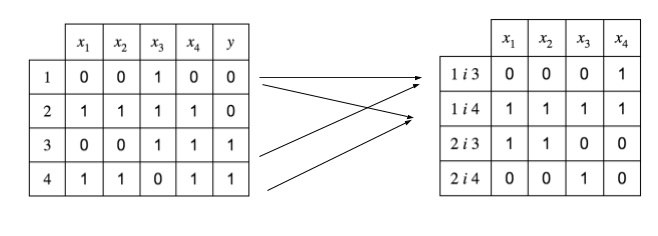
\includegraphics[width = 13cm]{chapter02/discernibility-table.png}
\caption{Proces powstawania tablicy rozróżnialności (Źródło własne).}
\end{figure}

Znalezienie reduktu,
przy użyciu tablicy rozróżnialności sprowadza się do problemu znalezienia minimalnego pokrycia kolumnowego,
czyli takiego zbioru kolumn,
dla którego w każdym z wierszy znajduje się co najmniej jedna jedynka.
Najprostszy algorytm znajdujący rozwiązanie sprowadzałby się do następujących kroków:
\begin{enumerate}
\item Wybranie kolumny o największej liczbie jedynek,
\item Usunięcie wierszy z jedynkami w tej kolumnie,
\item Powtarzanie aż do uzyskania pustej macierzy.
\end{enumerate}
Nie uwzględnia on jednak rozróżnień,
które są dostarczane przez niewielką liczbę argumentów.
Najłatwiej zauważyć to na przykładzie argumentów niezbędnych.
W ich przypadku istnieje taki wiersz,
który zawiera wyłącznie jedną jedynkę.
Oznacza to,
że argument odpowiadający tej jedynce jest niezbędny do uzyskania minimalnego pokrycia kolumnowego.
Taki argument często dostarcza innych rozróżnień,
które przy użyciu proponowanego algorytmu zawyżałyby sztucznie wartość innych argumentów.

\begin{figure}[H]
\centering
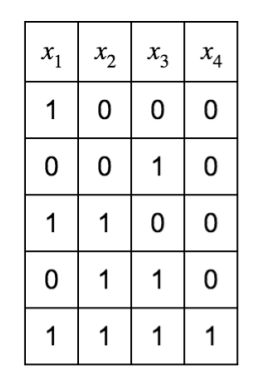
\includegraphics[width = 5cm]{chapter02/required-arguments.png}
\caption{Przykład obrazujący niedoskonałości algorytmu największej liczby jedynek.
Argument $x_2$ posiada najwięcej jedynek i jednocześnie jest nadmiarowy. (Źródło własne).}
\end{figure}

Aby uwzględnić ten problem,
w ostatecznym rozwiązaniu sposób wyboru kolumny jest dwuetapowy.
Najpierw znajdowany jest wiersz o najmniejszej liczbie jedynek,
następnie wybierana jest kolumna,
która ma najwięcej jedynek oraz jedynkę w wybranym wierszu.
Takie rozwiązanie wyboru kolumn jest optymalne i często prowadzi do uzyskania reduktu o najmniejszej liczności \cite{unate-artykul}.
Niestety w bardzo specyficznych przypadkach końcowe minimalne pokrycie kolumnowe również zawiera nadmiarowe argumenty.
Z tego powodu wymagane jest przeprowadzenie weryfikacji rozwiązania.


\begin{algorithm}[H]
    \KwData{$F$}
    \KwResult{$R$}
    $MR\gets$ pusta\;
    \For{dla każdej pary wierszy $F$ o różnej wartosci}{
        $W\gets$ wykonaj operację XOR poszczególnych bitów\;
        $MR\gets MR + W$\;
    }
    $MR2\gets MR$\;
    \While{$MR2$ niepusta}{
        \For{dla każdego wiersza $MR2$}{
            $W\gets$ znajdź wiersz o najmniejszej liczbie jedynek\;
        }
        \For{dla kolumn z jedynekami w $W$}{
            $K\gets$ znajdź kolumnę o największej liczbie jedynek\;
        }
        $R\gets R + K$\;
        \For{dla każdego wiersza $W$ w $MR2$}{
            \If{$W$ zawiera jedynkę na $K$}{
                $MR2\gets MR2 - W$\;
            }
        }
    }
    \For{dla każdego argumentu $K$ w $R$}{
        \If{$MR$ dla argumentów z $R$ bez $K$ jest spójna}{
            $R\gets R - K$\;
        }
    }
\end{algorithm}

Dla takiej samej funkcji o $n$ argumentach i $m$ wierszach złożoność obliczeniowa tworzenia tablicy rozróżnialności wynosi $n \cdot m^2$.
Następne kroki algorytmu operują na macierzy rozróżnialności,
dlatego przy szacowaniu ich złożoności musimy pamiętać o tym,
że tablica ma $m^2$ wierszy.
Także kolejne złożoności znajdowania wiersza o najmniejszej liczbie jedynek oraz kolumny o największej liczbie jedynek wynoszą $n \cdot m^2$ każda.
Maksymalna liczba powtórzeń,
dla funkcji nieredukowalnej,
wynosi $n$.
Warto pamiętać,
że każdy kolejny krok jest wykonywany dla pomniejszonej liczby wierszy,
ale na potrzeby szacowania złożoności przyjmijmy skrajnie niekorzystny przykład,
gdzie każdy argument usuwa tylko po jednym wierszu.
W takim przypadku bardzo pesymistycznie oszacowana złożoność wyniesie $n^2 \cdot m^2$.
Ostatni krok ma taką złożoność jak poprzednio liczona złożoność weryfikacji.
Ponownie warto zauważyć,
że obliczenia przeprowadzane są już na redukcie,
czyli zbiorze argumentów często mniejszym od $n$.
Podsumowując końcowa złożoność obliczeniowa wynosi $n \cdot m^2 + n^2 \cdot m^2 + n^2 \cdot m^2$,
czyli w dalszym ciągu $n^2 \cdot m^2$.
Wynika stąd,
że dzięki takiemu podejściu udało się uzyskać statystycznie lepszy redukt przy takiej samej złożoności obliczeniowej.


\section{Problem macierzy rozróżnialności}

W czasie przeprowadzania badań otrzymana złożoność nie stanowiła problemu.
Warto jednak zauważyć,
że rozmiar tablicy porównań dla bazy sygnatur wirusów o 1,3 mln wierszy,
byłby zbyt duży dla większości komputerów.
Jeżeli za rozmiar pojedynczego wiersza przyjęlibyśmy 5 bajtów (40 bitów), to o ile sama baza zajmowałaby około 6 MB pamięci to tablica porównań około 8 TB.

Taka złożoność pamięciowa jest niepraktyczna nie tylko w tym konkretnym przypadku,
ale również w wielu innych również poza domeną generowania indeksów.
Powstały z tego powodu algorytmy niewymagające generowania tablicy porównań.
Jednym z nich jest algorytm Marcina Korzenia i Szymona Jaroszewicza dokładnie przedstawiony w artykule \cite{without-matrix}.

Przy zastosowaniu ich rozwiązania można policzyć liczbę jedynek w kolumnach tablicy rozróżnialności z praw kombinatoryki.
W artykule przedstawione zostały obliczenia dla bardzo ogólnej bazy danych,
jednak w ramach tej pracy,
istotny jest jedynie przypadek funkcji zawierającej wyłącznie zera i jedynki wśród wartości argumentów.
Jedynka w kolumnie macierzy rozróżnialności powstaje,
kiedy dwa wiersze o różnej wartości funkcji mają różną wartość argumentu.
Taka suma przy uwzględnieniu jedynie dwóch możliwych wartości argumentu i kilku wartości funkcji jest stosunkowo łatwa do wyznaczenia.
W przypadku ogólnym poruszanym w artykule jest jednak dużo łatwiej policzyć,
kiedy jedynka nie występuje w tablicy i odjąć tę liczbę od liczby wierszy w macierzy.
Co więcej,
ponieważ liczba wierszy jest identyczna dla każdej kolumny,
obliczanie liczby wierszy nie jest potrzebne.
Wystarczy zastosować odwrotne podejście przy wyborze kolumny i wybierać te o najmniejszej liczbie zer.

Jeżeli podzielimy wiersze danych na grupy ze względu na wartość funkcji i argumentu,
powstaną po dwa kubełki dla każdej wartości funkcji.
Jeżeli ich rozmiar oznaczymy $K_{0_d}$ i $K_{1_d}$,
 gdzie $0$ i $1$ oznaczają wartość argumentu,
a $d$ należy do zbioru wartości funkcji,
liczbę zer w kolumnie można wyrazić następującą sumą:
\begin{equation}
\sum_{0<d_1<d_2<D} K_{0_{d_1}} \cdot K_{0_{d_2}} + K_{1_{d_1}} \cdot K_{1_{d_2}}
\end{equation}
Obliczenie wyznacznika ma w takim wypadku złożoność pamięciową liniowo zależną od liczby wartości funkcji,
czyli pomijalnie małą.
Innymi słowy, skutecznie rozwiązuje to problem pamięci zajmowanej przez tablicę rozróżnialności.
Dodatkowo mniejsza jest złożoność obliczeniowa.
Znalezienie najlepszej kolumny do uwzględnienia w redukcie odbywa się ze złożonością $n \cdot m$ w porównaniu do poprzedniego $n \cdot m^2$.

Takie rozwiązanie nie uwzględnia jednak argumentów niezbędnych i czasami będzie prowadzić do mniej optymalnych wyników niż algorytm użyty w niniejszej pracy.
Gdyby jednak dalsze badania lub konkretne zastosowania wymagały operacji na dużych bazach danych,
wymagane byłoby użycie tego lub podobnego algorytmu o mniejszej złożoności pamięciowej.

\section{Rozwiązania systematyczne}

Żadne z przedstawionych do tej pory rozwiązań nie było systematyczne.
Wszystko ze względu na zdecydowanie większą złożoność obliczeniową takich algorytmów.
W przypadku problemu generowania indeksów dane,
dla których przeprowadza się obliczenia,
zmieniają się w czasie,
dlatego czas tych obliczeń jest bardzo istotny.
Są jednak inne problemy,
w których czas optymalizacji nie jest czynnikiem istotnym.
Do takich zastosowań należą problemy dziedziny eksploracji danych,
gdzie często dane są zbierane na długo przed przeprowadzeniem obliczeń,
lub implementacji funkcji w układach FPGA czy też innych z pamięciami ROM.

W zadaniach, gdzie na wynik obliczeń możemy poczekać oraz nawet najmniejsza optymalizacja końcowego wyniku jest istotna,
rozwiązania systematyczne pokazują prawdziwą potęgę.
Na przykładzie redukcji argumentów,
takie algorytmy nie tylko dostarczają zawsze najmniejszy redukt,
ale wszystkie najmniejsze redukty.
Otwierają więc możliwość przeprowadzenia dalszych optymalizacji (np. kompresji argumentów) z różnymi danymi początkowymi pozornie równie dobrymi.

\section{Unate Complement}

Ze względu na to,
że algorytmy systematyczne dostarczają wszystkich rozwiązań,
mogą w czasie badań służyć do weryfikacji jakości rozwiązań pochodzących z algorytmów heurystycznych.
Algorytmem użytym w tym celu w ramach pracy był algorytm Unate Complement.

Algorytm Unate Complement służy do wyznaczania dopełnienia funkcji jednorodnej,
czyli takiej,
dla której w żadnej kolumnie nie występują jednocześnie zera i jedynki.
Tym samym pozwala na znalezienie wszystkich największych (najbardziej ogólnych) kostek dopełnienia funkcji jednorodnej,
a zastosowany do tablicy porównań pozwala na wyznaczenie wszystkich minimalnych pokryć kolumnowych.

Sam algorytm składa się z czterech kroków:
\begin{enumerate}
\item Rekurencyjnego rozkładu funkcji zgodnie ze wzorem Shannona,
\item Obliczania dopełnień w liściach zgodnie z prawami De Morgana,
\item Rekurencyjnego łączenia powstałych dopełnień ponownie przy wykorzystaniu wzoru Shannona,
\item Usunięcia nadmiarowych reduktów,
czyli takich,
które zawierają się w innych zgodnie z rachunkiem kostek.
\end{enumerate}
Badania nad tym algorytmem zostały opisane w pracy inżynierskiej \cite{inzynierka},
a gotowy program służył do weryfikacji poprawności działania użytego algorytmu redukcji argumentów.



\backmatter
\pagestyle{empty}
%%*******************************************************************************
% Bibliografia - spis literatury wykorzystanej przy tworzeniu pracy
%*******************************************************************************

\begin{thebibliography}{99}
\addcontentsline{toc}{chapter}{Bibliografia}
\bibliographystyle{tran}

%[1] Borowik G., Łuba T.: Fast Algorithm of Attribute Reduction Based on the complementation of Boolean Function, ch. 2, pp. 25-41, Springer International Publishing, 2014.
\bibitem{fast-algorithm} G. Borowik, T. Łuba \emph{,,Fast Algorithm of Attribute Reduction Based on the complementation of Boolean Function''}, ch. 2, pp. 25-41, Springer International Publishing, 2014.

%[2] G. Borowik, K. Kowalski: Efektywna procedura uzupełnienia funkcji boolowskich i jej zastosowaniew eksploracji danych. Przegląd Telekomunikacyjny i Wiadomości Telekomunikacyjne. 03/2015.
\bibitem{efektywna-procedura} G. Borowik, K. Kowalski \emph{,,Efektywna procedura uzupełnienia funkcji boolowskich i jej zastosowanie w eksploracji danych''}, Przegląd Telekomunikacyjny i Wiadomości Telekomunikacyjne, 03/2015.

\bibitem{inzynierka} K. Kowalski \emph{,,Implementacja Algorytmu Uzupełnienia Funkcji Boolowskich z Wykorzystaniem Programowania Współbieżnego''}, Praca Dyplomowa Inżynierska, 2014.

%[3] Chen, D., Wang, C., Hu, Q., 2007. A new approach to attribute reduction of consistent and inconsistent covering decision systems with covering rough sets. Information Sciences 177, 3500–3518.
\bibitem{new-reduction} D. Chen, C. Wang, Q. Hu \emph{,,A new approach to attribute reduction of consistent and inconsistent covering decision systems with covering rough sets''}, Information Sciences 177, 3500–3518, 2007.

%[4] Łuba T., Borowik G.: Synteza logiczna, Oficyna Wydawnicza PW, Warszawa 2015.
\bibitem{synteza-logiczna} T. Łuba, G. Borowik \emph{,,Synteza logiczna''}, Oficyna Wydawnicza PW, Warszawa 2015.

%[5] Łuba T., Poźniak K., Zbierzchowski B.: Redukcja i kompresja zmiennych w syntezie funkcji generowania indeksów. Przegląd telekomunikacyjny, nr. 10, 2016.
\bibitem{redukcja-kompresja} T. Łuba, K. Poźniak, B. Zbierzchowski \emph{,,Redukcja i kompresja zmiennych w syntezie funkcji generowania indeksów''}, Przegląd telekomunikacyjny, nr. 10, 2016.

%[6] Łuba, T., Rybnik J.:  Algorithmic Approach to Discernibility Function with Respect to Attributes and Objects Reduction, Foundations of Computing and Decision Sciences, Vol. 18, No. 3-4, 241–258, 1993.
\bibitem{algorithmic-approach} T. Łuba, J. Rybnik \emph{,,Algorithmic Approach to Discernibility Function with Respect to Attributes and Objects Reduction''}, Foundations of Computing and Decision Sciences, Vol. 18, No. 3-4, 241–258, 1993.

%[7] Sasao T.: Index Generation Functions, Logic Synthesis for Pattern Matching, EPFL Workshop on Logic Synthesis & Verification, Dec. 2015.
\bibitem{sasao-workshop} T. Sasao \emph{,,Index Generation Functions''}, Logic Synthesis for Pattern Matching, EPFL Workshop on Logic Synthesis \& Verification, Dec. 2015.

%[8] Sasao, T.: Index generation functions: Recent developments,  International Symposium on Multiple-Valued Logic (ISMVL-2011), Tuusula, Finland, May 2011.
\bibitem{sasao-recent} T. Sasao \emph{,,Index generation functions: Recent developments''}, International Symposium on Multiple-Valued Logic (ISMVL-2011), Tuusula, Finland, May 2011.

%[9] Sasao, T.:  A Reduction Method For the Number of Variables to Represent Index Generation Functions: s-Min Method, IEEE 45th International Symposium on Multiple-Valued Logic, 164–169, 2015.
\bibitem{sasao-s-min} T. Sasao \emph{,,A Reduction Method For the Number of Variables to Represent Index Generation Functions: s-Min Method''}, IEEE 45th International Symposium on Multiple-Valued Logic, 164–169, 2015.

%[10] Sasao, T.: Memory-Based Logic Synthesis, Springer New York Dordrecht Heidelberg London, 2011.
\bibitem{sasao-synthesis} T. Sasao \emph{,,Memory-Based Logic Synthesis''}, Springer New York Dordrecht Heidelberg London, 2011.

%[11] RSES – Rough Set Exploration System, http://logic.mimuw.edu.pl/~rses/
\bibitem{rses} \emph{,,RSES – Rough Set Exploration System''} [Online] http://logic.mimuw.edu.pl/~rses/

%[12] Steinbach B., Posthoff C., Improvements of the Construction of Exact Minimal Covers of Boolean Functions, Computer Aided Systems Theory – EUROCAST 2011, Lecture Notes in Computer Science Volume 6928, pp. 272-279, 2012.
\bibitem{steinbach-posthoff} B. Steinbach, C. Posthoff \emph{,,Improvements of the Construction of Exact Minimal Covers of Boolean Functions''}, Computer Aided Systems Theory – EUROCAST 2011, Lecture Notes in Computer Science Volume 6928, pp. 272-279, 2012.

%[13] Skowron, A., Rauszer, C., 1992. The discernibility matrices and functions in information systems, in: Słowiński, R. (Ed.), Intelligent Decision Support. Springer Netherlands. volume 11 of Theory and Decision Library, pp. 331– 362.
\bibitem{skowron-rauszer} A. Skowron, C. Rauszer \emph{,,The discernibility matrices and functions in information systems''}, Słowiński, R. (Ed.), Intelligent Decision Support. Springer Netherlands. volume 11 of Theory and Decision Library, pp. 331– 362, 1992.

%[14] Ślezak, D., 1998. Searching for dynamic reducts in inconsistent decision tables,  in: Proceedings of IPMU 98, pp. 1362–1369.
\bibitem{slezak} D. Ślezak \emph{,,Searching for dynamic reducts in inconsistent decision tables''}, Proceedings of IPMU 98, pp. 1362–1369. 1998.

%[15] Wang, C., He, Q., Chen, D., Hu, Q., 2014. A novel method for attribute reduction of covering decision systems. Information Sciences 254, 181–196.
\bibitem{novel-method} C. Wang, Q. He, D. Chen, Q. Hu \emph{,,A novel method for attribute reduction of covering decision systems''}, Information Sciences 254, 181–196, 2014.

\bibitem{unate-artykul} T. Łuba, G. Borowik, K. Kowalski, P. Pecio, C. Jankowski, M. Mańkowski \emph{,,Rola i znaczenie syntezy logicznej w eksploracji danych dla potrzeb telekomunikacji i medycyny''}, Przegląd Telekomunikacyjny, str. 110-116, 05/2014.

\bibitem{without-matrix} M. Korzeń, S. Jaroszewicz \emph{,,Finding Reducts Without Building the Discernibility Matrix''}, Intelligent Systems Design and Applications, 2005.

\end{thebibliography}
\clearpage




%===============================================================================
							% bibliografia

%===============================================================================
% Koniec

%%*******************************************************************************
% Bibliografia - spis literatury wykorzystanej przy tworzeniu pracy
%*******************************************************************************

\begin{thebibliography}{99}
\addcontentsline{toc}{chapter}{Bibliografia}
\bibliographystyle{tran}

%[1] Borowik G., Łuba T.: Fast Algorithm of Attribute Reduction Based on the complementation of Boolean Function, ch. 2, pp. 25-41, Springer International Publishing, 2014.
\bibitem{fast-algorithm} G. Borowik, T. Łuba \emph{,,Fast Algorithm of Attribute Reduction Based on the complementation of Boolean Function''}, ch. 2, pp. 25-41, Springer International Publishing, 2014.

%[2] G. Borowik, K. Kowalski: Efektywna procedura uzupełnienia funkcji boolowskich i~jej zastosowaniew eksploracji danych. Przegląd Telekomunikacyjny i~Wiadomości Telekomunikacyjne. 03/2015.
\bibitem{efektywna-procedura} G. Borowik, K. Kowalski \emph{,,Efektywna procedura uzupełnienia funkcji boolowskich i~jej zastosowanie w~eksploracji danych''}, Przegląd Telekomunikacyjny i~Wiadomości Telekomunikacyjne, 03/2015.

\bibitem{inzynierka} K. Kowalski \emph{,,Implementacja Algorytmu Uzupełnienia Funkcji Boolowskich z~Wykorzystaniem Programowania Współbieżnego''}, Praca Dyplomowa Inżynierska, 2014.

%[3] Chen, D., Wang, C., Hu, Q., 2007. A~new approach to attribute reduction of consistent and inconsistent covering decision systems with covering rough sets. Information Sciences 177, 3500–3518.
\bibitem{new-reduction} D. Chen, C. Wang, Q. Hu \emph{,,A new approach to attribute reduction of consistent and inconsistent covering decision systems with covering rough sets''}, Information Sciences 177, 3500–3518, 2007.

%[4] Łuba T., Borowik G.: Synteza logiczna, Oficyna Wydawnicza PW, Warszawa 2015.
\bibitem{synteza-logiczna} T. Łuba, G. Borowik \emph{,,Synteza logiczna''}, Oficyna Wydawnicza PW, Warszawa 2015.

%[5] Łuba T., Poźniak K., Zbierzchowski B.: Redukcja i~kompresja zmiennych w~syntezie funkcji generowania indeksów. Przegląd telekomunikacyjny, nr. 10, 2016.
\bibitem{redukcja-kompresja} T. Łuba, K. Poźniak, B. Zbierzchowski \emph{,,Redukcja i~kompresja zmiennych w~syntezie funkcji generowania indeksów''}, Przegląd telekomunikacyjny, nr. 10, 2016.

%[6] Łuba, T., Rybnik J.:  Algorithmic Approach to Discernibility Function with Respect to Attributes and Objects Reduction, Foundations of Computing and Decision Sciences, Vol. 18, No. 3-4, 241–258, 1993.
\bibitem{algorithmic-approach} T. Łuba, J. Rybnik \emph{,,Algorithmic Approach to Discernibility Function with Respect to Attributes and Objects Reduction''}, Foundations of Computing and Decision Sciences, Vol. 18, No. 3-4, 241–258, 1993.

%[7] Sasao T.: Index Generation Functions, Logic Synthesis for Pattern Matching, EPFL Workshop on Logic Synthesis & Verification, Dec. 2015.
\bibitem{sasao-workshop} T. Sasao \emph{,,Index Generation Functions''}, Logic Synthesis for Pattern Matching, EPFL Workshop on Logic Synthesis \& Verification, Dec. 2015.

%[8] Sasao, T.: Index generation functions: Recent developments,  International Symposium on Multiple-Valued Logic (ISMVL-2011), Tuusula, Finland, May 2011.
\bibitem{sasao-recent} T. Sasao \emph{,,Index generation functions: Recent developments''}, International Symposium on Multiple-Valued Logic (ISMVL-2011), Tuusula, Finland, May 2011.

%[9] Sasao, T.:  A~Reduction Method For the Number of Variables to Represent Index Generation Functions: s-Min Method, IEEE 45th International Symposium on Multiple-Valued Logic, 164–169, 2015.
\bibitem{sasao-s-min} T. Sasao \emph{,,A Reduction Method For the Number of Variables to Represent Index Generation Functions: s-Min Method''}, IEEE 45th International Symposium on Multiple-Valued Logic, 164–169, 2015.

%[10] Sasao, T.: Memory-Based Logic Synthesis, Springer New York Dordrecht Heidelberg London, 2011.
\bibitem{sasao-synthesis} T. Sasao \emph{,,Memory-Based Logic Synthesis''}, Springer New York Dordrecht Heidelberg London, 2011.

%[11] RSES – Rough Set Exploration System, http://logic.mimuw.edu.pl/~rses/
\bibitem{rses} \emph{,,RSES – Rough Set Exploration System''} [Online] http://logic.mimuw.edu.pl/~rses/

%[12] Steinbach B., Posthoff C., Improvements of the Construction of Exact Minimal Covers of Boolean Functions, Computer Aided Systems Theory – EUROCAST 2011, Lecture Notes in Computer Science Volume 6928, pp. 272-279, 2012.
\bibitem{steinbach-posthoff} B. Steinbach, C. Posthoff \emph{,,Improvements of the Construction of Exact Minimal Covers of Boolean Functions''}, Computer Aided Systems Theory – EUROCAST 2011, Lecture Notes in Computer Science Volume 6928, pp. 272-279, 2012.

%[13] Skowron, A., Rauszer, C., 1992. The discernibility matrices and functions in information systems, in: Słowiński, R. (Ed.), Intelligent Decision Support. Springer Netherlands. volume 11 of Theory and Decision Library, pp. 331– 362.
\bibitem{skowron-rauszer} A. Skowron, C. Rauszer \emph{,,The discernibility matrices and functions in information systems''}, Słowiński, R. (Ed.), Intelligent Decision Support. Springer Netherlands. volume 11 of Theory and Decision Library, pp. 331– 362, 1992.

%[14] Ślezak, D., 1998. Searching for dynamic reducts in inconsistent decision tables,  in: Proceedings of IPMU 98, pp. 1362–1369.
\bibitem{slezak} D. Ślezak \emph{,,Searching for dynamic reducts in inconsistent decision tables''}, Proceedings of IPMU 98, pp. 1362–1369. 1998.

%[15] Wang, C., He, Q., Chen, D., Hu, Q., 2014. A~novel method for attribute reduction of covering decision systems. Information Sciences 254, 181–196.
\bibitem{novel-method} C. Wang, Q. He, D. Chen, Q. Hu \emph{,,A novel method for attribute reduction of covering decision systems''}, Information Sciences 254, 181–196, 2014.

\bibitem{unate-artykul} T. Łuba, G. Borowik, K. Kowalski, P. Pecio, C. Jankowski, M. Mańkowski \emph{,,Rola i~znaczenie syntezy logicznej w~eksploracji danych dla potrzeb telekomunikacji i~medycyny''}, Przegląd Telekomunikacyjny, str. 110-116, 05/2014.

\bibitem{without-matrix} M. Korzeń, S. Jaroszewicz \emph{,,Finding Reducts Without Building the Discernibility Matrix''}, Intelligent Systems Design and Applications, 2005.

\bibitem{memory-capacity} G. Borowik, T. Łuba, P. Tomaszewicz \emph{,,On the Memory Capacity to Implement Logic Functions''}, Eds. F. Pichler, R. Moreno-Díaz, A. Quesada-Arencibia, Computer Aided Systems Theory – EUROCAST 2011, vol.6928: Springer-Verlag Berlin Heidelberg, Lecture Notes in Computer Science, 343-350, 2012.

\bibitem{nine-filters} D.J.Goodman, M.J. Carey \emph{,,Nine Digital Filters for Decimation and Interpolation''}, IEEE Trans. On Acoustics, Speech and Signal Processing 25(2), pp.121-126, 1977.

\bibitem{redukcja-kompresja} T. Łuba, K. Poźniak, B. Zbierzchowski \emph{,,Redukcja i kompresja zmiennych w syntezie funkcji generowania indeksów''}, Przegląd Telekomunikacyjny i Wiadomości Telekomunikacyjne, pp. 1230 - 1236, Nr. 10/2016.

\bibitem{wirusy} H. Nakahara, T. Sasao, M. Matsuura, Y. Kawamura, \emph{,,A parallel sieve method for a virus scanning engine''}, 12th EUROMICRO Conference on Digital System Design, Architectures, Methods and Tools, Patras, Greece (DSD-2009), Aug. 2009, pp.809-816.

\end{thebibliography}
\clearpage




%===============================================================================


\chapter*{Wykaz symboli i skrótów}
\addcontentsline{toc}{chapter}{Wykaz symboli i skrótów}

\noindent
\textbf{F} - funkcja, \newline
\textbf{G} - wejściowa składowa dekompozycji, \newline
\textbf{H} - wyjsciowa składowa dekompozycji, \newline
\textbf{k} - liczba wierszy funkcji, \newline
\textbf{MR} - macierz rozróżnialności, \newline
\textbf{m} - liczba wierszy funkcji, \newline
\textbf{n} - liczba argumentów funkcji, \newline
\textbf{R} - redukt, \newline
\textbf{\texorpdfstring{w\textsubscript{i}}}{ - i-ty wiersz funckji,}\newline
\textbf{X} - zbiór argumentów, \newline
\textbf{\texorpdfstring{x\textsubscript{i}}{x i}} - i-ty argument funckji, \newline
\textbf{\texorpdfstring{x\textsubscript{i\textsubscript{w\textsubscript{j}}}}{x i w j}} - wartość i-tego argumentu dla j-tego wiersza w funkcji, \newline
\textbf{Y} - zbiór wartości funkcji, \newline
\textbf{\texorpdfstring{y\textsubscript{i}}{y i}} - i-ta wrtość funkcji, \newline

\cleardoublepage

\listoffigures
\addcontentsline{toc}{chapter}{Spis rysunków}
\cleardoublepage

\listoftables
\addcontentsline{toc}{chapter}{Spis tablic}
\cleardoublepage

%Spis załączników

%Załączniki

\end{document}

%===============================================================================
